\documentclass[12pt, a4paper]{article}

\usepackage[hmargin=2.5cm, vmargin=2cm]{geometry}
\usepackage{amsthm, amssymb, mathtools, yhmath, graphicx}
\usepackage{fontspec, type1cm, titlesec, titling, fancyhdr, tabularx}
\usepackage{color, unicode-math, float, hhline}

\usepackage[CheckSingle, CJKmath]{xeCJK}
\usepackage{CJKulem}
\usepackage{enumitem}
\usepackage{tikz}
%\usepackage{circuitikz}
\usepackage{minted}
\usepackage{pifont}
\usepackage{PTSansNarrow}
%\usepackage[T1]{fontenc}
\setmainfont{Linux Libertine O}
\setmonofont{Source Code Pro}
\usetikzlibrary{matrix}
%\setCJKmainfont[BoldFont=cwTex Q Hei]{cwTex Q Ming}
%\setCJKsansfont[BoldFont=cwTex Q Hei]{cwTex Q Ming}
%\setCJKmonofont[BoldFont=cwTex Q Hei]{cwTex Q Ming}
%\setCJKmainfont[BoldFont=cwTeX Q Hei]{cwTeX Q Ming}
%\setCJKmainfont{Source Han Sans TWHK}
\setCJKmainfont{Source Han Sans TC}

\def\normalsize{\fontsize{12}{18}\selectfont}
\def\large{\fontsize{14}{21}\selectfont}
\def\Large{\fontsize{16}{24}\selectfont}
\def\LARGE{\fontsize{18}{27}\selectfont}
\def\huge{\fontsize{20}{30}\selectfont}

%\titleformat{\section}{\bf\Large}{\arabic{section}}{24pt}{}
%\titleformat{\subsection}{\large}{\arabic{subsection}.}{12pt}{}
%\titlespacing*{\subsection}{0pt}{0pt}{1.5ex}

\parindent=24pt

\DeclarePairedDelimiter{\abs}{\lvert}{\rvert}
\DeclarePairedDelimiter{\norm}{\lVert}{\rVert}
\DeclarePairedDelimiter{\inpd}{\langle}{\rangle}
\DeclarePairedDelimiter{\ceil}{\lceil}{\rceil}
\DeclarePairedDelimiter{\floor}{\lfloor}{\rfloor}

\newcommand{\img}{\mathsf{i}}
\newcommand{\ex}{\mathsf{e}}
\newcommand{\dD}{\mathrm{d}}
\newcommand{\dI}{\,\mathrm{d}}

\newcommand{\cmark}{\ding{51}}
\newcommand{\ftt}[1]{\framebox[1.3\width]{\texttt{#1}}}

\setminted[sv]{
  linenos=true, frame=lines, framesep=2mm
}

\title{數位電路實驗 Lab-1 使用手冊 -- 點名器}
\author{Team \#2}
\begin{document}
\maketitle

\section{概覽}
我們總共實做了兩個版本,一個是純 Verilog 實作的版本,另一個則是
由 Nios II CPU 做為主要的控置器的版本。

\section{功能簡介}
\begin{figure}[H]
  \centering
  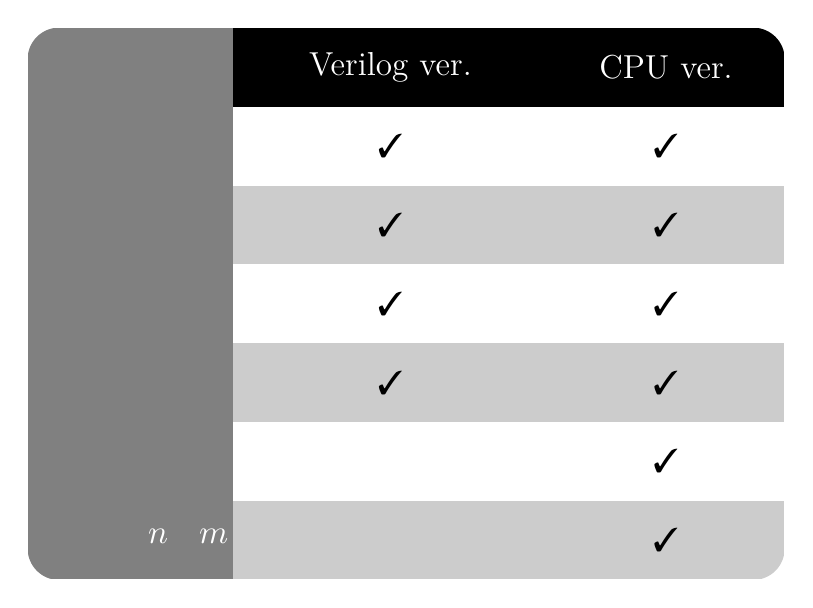
\begin{tikzpicture}
  \clip node (m) [matrix,matrix of nodes,
  fill=black!20,inner sep=0pt,
  nodes in empty cells,
  nodes={minimum height=1cm,minimum width=2.6cm,anchor=center,outer sep=0},
  row 1/.style={nodes={fill=black,text=white}},
  column 1/.style={nodes={fill=gray,text=white,align=right,text width=2.5cm,text depth=0.5ex}},
  column 2/.style={text width=4cm,align=center,every even row/.style={nodes={fill=white}}},
  column 3/.style={text width=3cm,align=center,every even row/.style={nodes={fill=white}},},
  row 1 column 1/.style={nodes={fill=gray}},
  prefix after command={[rounded corners=4mm] (m.north east) rectangle (m.south west)}
  ] {
                  & Verilog ver.                     & CPU ver. \\
  亂數            & \cmark & \cmark \\
  數字跳動        & \cmark & \cmark \\
  結束特效        & \cmark & \cmark \\
  重新開始        & \cmark & \cmark \\
  數字上限        & & \cmark \\
  $n$ 選 $m$      & & \cmark \\
  };
  \end{tikzpicture}
\end{figure}

以下詳述這些功能的內容。
\begin{enumerate}
  \item {\bf 亂數} \\
    在 Verilog 的版本,我們實作了一個 Linear congruential generator 的 Pseudo random number generator。
    而在 CPU 版本,我們直接使用內建的函式 $\texttt{rand}$。

    為了確保重新開機後,每次產生的亂數不同,我們最後選出的數字會和使用者按下開始的時間有關。

  \item {\bf 數字跳動} \\
    在最終的數字被選出之前,LED 的數字會不斷跳動,並且跳動的速度會漸漸變慢
    ,這樣似乎會有一種比較刺激的感覺(?)

  \item {\bf 結束特效} \\
    在最終的數字被選出之後 LED 會閃爍數次提示使用者。

  \item {\bf 重新開始} \\
    機器不需要重新開機即可進行下一次的點名。

  \item {\bf 數字上限} \\
    可以手動設定數字上限 $N$ , 產生出 $[1, N]$ 之間的數字,僅 CPU Ver. 有此功能。
    Verilog Ver. 固定產生的數字範圍是 $[0, 15]$。
    
  \item {\bf $n$ 選 $m$} \\
    可以手動設定要抽出幾個號碼,並且抽出的這些號碼不會重複,
    流程結束後 LED 也會不斷的循環播放所有抽出的數字。
    僅 CPU Ver. 有此功能。
\end{enumerate}

\section{使用說明}
\begin{figure}[H]
  \centering
  \begin{tikzpicture}
    \node at (0, 0) {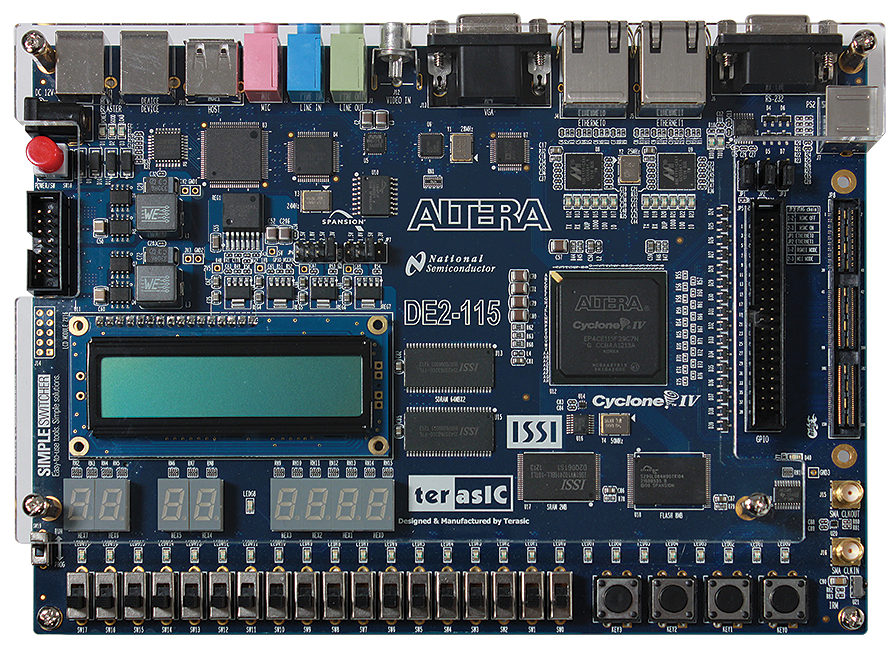
\includegraphics[width=.75\textwidth]{figure/DE2_115.png}};
    \draw[red, very thick] (-1.52, -2.7) rectangle (-0.7, -2.0);
    \draw[red, very thick] (-3.9, -2.7) rectangle (-3.02, -2.0);
    \draw[red, very thick] (-5.15, -2.7) rectangle (-4.26, -2.0);

    \draw[red, very thick, -latex] (-1.11, -2.8) -- (-1.11, -5) node[below]{\texttt{L0}};
    \draw[red, very thick, -latex] (-3.46, -2.8) -- (-3.46, -5) node[below]{\texttt{L1}};
    \draw[red, very thick, -latex] (-4.70, -2.8) -- (-4.70, -5) node[below]{\texttt{L2}};

    \draw[red, very thick, -latex] (2.3, -4.1) -- (2.3, -5) node[below]{\texttt{B2}};
    \draw[red, very thick, -latex] (3.04, -4.1) -- (3.04, -5) node[below]{\texttt{B1}};
    \draw[red, very thick, -latex] (3.78, -4.1) -- (3.78, -5) node[below]{\texttt{B0}};
    \draw[red, very thick, -latex] (4.52, -4.1) |- (5.2, -4.8) node[right]{\texttt{RST}};
  \end{tikzpicture}
\end{figure}

\subsection{Verilog Ver.}
\begin{enumerate}
  \itemsep=0pt
  \item 按下 \ftt{RST} 按鈕後點名器即開始抽出號碼。
  \item \ftt{L0} 上的數字會開始不斷跳動,並漸漸變慢。
  \item 等到 \ftt{L0} 上的數字停止時,\ftt{L0} 會閃爍。 此時
    顯示的數字即為被抽到的數字。
  \item 接下來可以再次按下 \ftt{RST} 鍵再次執行選號。
\end{enumerate}

\subsection{CPU Ver.}
開機後,系統會進入待機模式等待使用者。
\subsubsection{重設}
\begin{enumerate}
  \itemsep=0pt
  \item 按下 \ftt{RST} 鍵可以重設機器,所有儲存的狀態都會消失。
\end{enumerate}

\subsubsection{設定參數}
總共有兩個選項可以供使用者調整。
\begin{enumerate}
  \itemsep=0pt
  \item {\bf 數字的範圍 $N$}: 抽出的數字會在 $[1, N]$ 之間。
  \item {\bf 抽選的數字 $C$}: 總共抽出 $C$ 個數字。 系統會自動限制 $1 \leq C \leq N$。
\end{enumerate}
在待機模式下 \ftt{L2} 會顯示 $N$, \ftt{L1} 會顯示 $C$ 。 \\

\noindent
設定的流程如下:
\begin{enumerate}
  \itemsep=0pt
  \item 在{\bf 待機模式}下按下 \ftt{B0} 按鈕後即會進入設定模式。
  \item \ftt{L2} 會閃爍,提示使用者是在更動 $N$。 此時使用者可以
    透過按鈕 \ftt{B1} 來增加 $N$,每按一次 $N$ 會增加 $1$。如果超
    過 $99$,$N, C$ 會自動回到 $1$。 可以長按按鈕來快速增加 $N$ 的
    值。
  \item 更改完成 $N$ 的值後,按一次 \ftt{B0} 確認。
  \item 此時換 \ftt{L1} 會閃爍,提示使用者是在更動 $C$。 使用者可以
    透過按鈕 \ftt{B1} 來增加 $C$,每按一次 $C$ 會增加 $1$。如果超
    過 $N$,$C$ 會自動回到 $1$。 可以長按按鈕來快速增加 $C$ 的
    值。
  \item 更改完成 $C$ 的值後,再按一次 \ftt{B0} 確認回到待機模式。
\end{enumerate}

\subsubsection{選號}
\begin{enumerate}
  \itemsep=0pt
  \item 按下 \ftt{B2} 按鈕後點名器即開始執行模式。
  \item \ftt{L2} 會顯示當前正在抽出第幾個數字。 
  \item \ftt{L0} 上的數字會開始不斷跳動,並漸漸變慢。 \label{proc-begin}
  \item 等到 \ftt{L0} 上的數字停止時,\ftt{L0} 會閃爍。 此時
    顯示的數字即為被抽到的數字。 \label{proc-end}
  \item 系統會重複執行步驟 \ref{proc-begin} -- \ref{proc-end} $C$ 次,抽
    出總共 $C$ 個數字。
  \item 流程結束後系統會回到待機模式。此時 \ftt{L0} 會不斷循環顯示上一次
    抽出的 $C$ 個數字。
\end{enumerate}

\end{document}

